\documentclass[12pt,a4paper]{scrartcl}\usepackage[]{graphicx}\usepackage[]{color}
%% maxwidth is the original width if it is less than linewidth
%% otherwise use linewidth (to make sure the graphics do not exceed the margin)
\makeatletter
\def\maxwidth{ %
  \ifdim\Gin@nat@width>\linewidth
    \linewidth
  \else
    \Gin@nat@width
  \fi
}
\makeatother

\definecolor{fgcolor}{rgb}{0.345, 0.345, 0.345}
\newcommand{\hlnum}[1]{\textcolor[rgb]{0.686,0.059,0.569}{#1}}%
\newcommand{\hlstr}[1]{\textcolor[rgb]{0.192,0.494,0.8}{#1}}%
\newcommand{\hlcom}[1]{\textcolor[rgb]{0.678,0.584,0.686}{\textit{#1}}}%
\newcommand{\hlopt}[1]{\textcolor[rgb]{0,0,0}{#1}}%
\newcommand{\hlstd}[1]{\textcolor[rgb]{0.345,0.345,0.345}{#1}}%
\newcommand{\hlkwa}[1]{\textcolor[rgb]{0.161,0.373,0.58}{\textbf{#1}}}%
\newcommand{\hlkwb}[1]{\textcolor[rgb]{0.69,0.353,0.396}{#1}}%
\newcommand{\hlkwc}[1]{\textcolor[rgb]{0.333,0.667,0.333}{#1}}%
\newcommand{\hlkwd}[1]{\textcolor[rgb]{0.737,0.353,0.396}{\textbf{#1}}}%
\let\hlipl\hlkwb

\usepackage{framed}
\makeatletter
\newenvironment{kframe}{%
 \def\at@end@of@kframe{}%
 \ifinner\ifhmode%
  \def\at@end@of@kframe{\end{minipage}}%
  \begin{minipage}{\columnwidth}%
 \fi\fi%
 \def\FrameCommand##1{\hskip\@totalleftmargin \hskip-\fboxsep
 \colorbox{shadecolor}{##1}\hskip-\fboxsep
     % There is no \\@totalrightmargin, so:
     \hskip-\linewidth \hskip-\@totalleftmargin \hskip\columnwidth}%
 \MakeFramed {\advance\hsize-\width
   \@totalleftmargin\z@ \linewidth\hsize
   \@setminipage}}%
 {\par\unskip\endMakeFramed%
 \at@end@of@kframe}
\makeatother

\definecolor{shadecolor}{rgb}{.97, .97, .97}
\definecolor{messagecolor}{rgb}{0, 0, 0}
\definecolor{warningcolor}{rgb}{1, 0, 1}
\definecolor{errorcolor}{rgb}{1, 0, 0}
\newenvironment{knitrout}{}{} % an empty environment to be redefined in TeX

\usepackage{alltt}
\usepackage[utf8]{inputenc}
\usepackage{amsmath}
\usepackage{graphicx}
\usepackage{tikz}
%\usepackage{silence}
\usepackage{mdframed}
%\WarningFilter{mdframed}{You got a bad break}
\usepackage[colorinlistoftodos]{todonotes}
\usepackage{listings}
\usepackage{color}
\colorlet{exampcol}{blue!10}
\usepackage{multicol}
\usepackage{booktabs}

\usepackage{exercise}

\usepackage[autostyle, english = american]{csquotes}
\MakeOuterQuote{"}

\usepackage{hyperref}
\hypersetup{
    colorlinks,
    citecolor=black,
    filecolor=black,
    linkcolor=blue,
    urlcolor=black
}

\title{Exercises for statistical inference and stuff}
\date{\today}
\author{Timoth\'ee Bonnet}
\IfFileExists{upquote.sty}{\usepackage{upquote}}{}
\begin{document}


\maketitle

\tableofcontents
\ListOfExerciseInToc
\ExerciseLevelInToc{subsubsection}

\clearpage

\section{Understanding error structure}

\subsection{Broken experiments}

\begin{Exercise}[difficulty=1, title={A significant result?}]
We carry out a vaccine challenge experiment. There are three experimental groups (saline control / low vaccine dose / high vaccine dose), with 6 mice in each group. For each group all mice are housed together in the same cage (so there are three cages). All mice are challenged with \emph{Shigella}, their symptom intensity is scored on day 8. A one-way ANOVA identifies an effect of the treatment, and pair-wise Bonferroni tests show the low-dose to be statistically significant different from the two other groups:

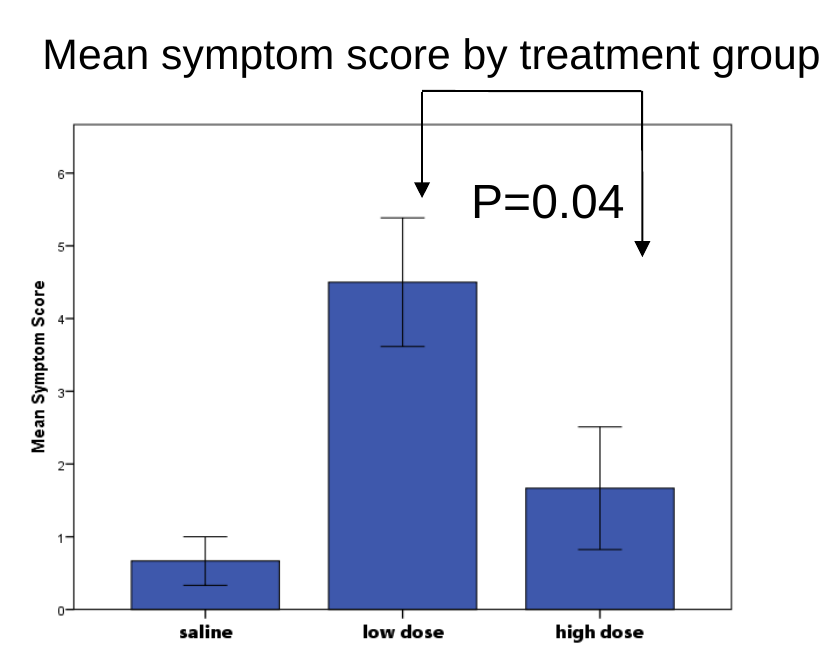
\includegraphics[width=0.4\textwidth]{Figures/message1}

\textbf{What is suspicious in the result? What part of the design may explain the result? How to improve the design (there are at least two different ways)?}
\end{Exercise}


\begin{Exercise}[difficulty=1, title={A better experimental design}]
We study how a membrane protein intakes external molecules in frog eggs. The target molecules are radioactively labelled so we can measure intake. We created five mutant lines to test what part of the protein controls intake. We propose to measure six tubes of ten eggs every week. Each week we will test a different genotype (i.e., the control or one of the five mutants):

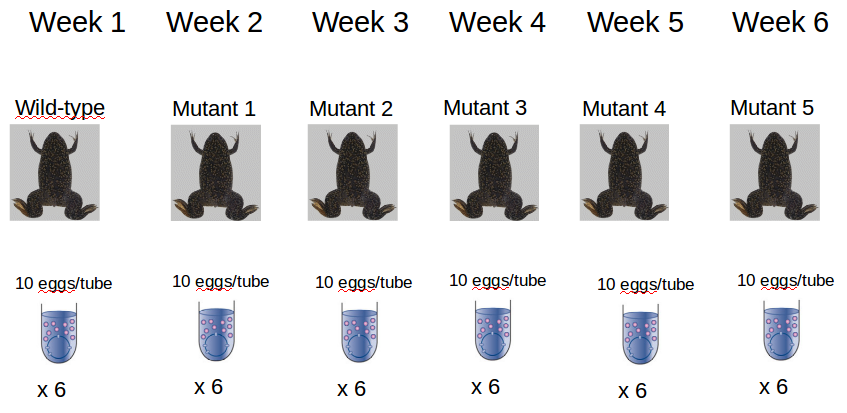
\includegraphics[width=0.8\textwidth]{Figures/expdes2}

\textbf{How much information about mutants can we extract from this experiment? How to improve the design?}

\end{Exercise}


\subsection{Broken models?}

Let's look at models with data from the an experiment similar to the mice example.
\begin{Exercise}[difficulty=1, title={lm vs. lmer vs. lm+}]

Load the dataset "challenge2.csv", and test the effect of the vaccine treatment ("Group") on the immune response ("Percent.loss"). 
First fit a fixed-effect only linear model and/or an anova. Is there a clear effect of treatment?\\
Now add a random effect for Cage (e.g., using the package lme4), what happens to the effect of treatment?\\
Finally, fit Cage and Group as fixed effects in a simple linear model and/or anova. What happens, why?\\
Which of the three models should you trust or not?

\end{Exercise}




\section{Interpreting simple mixed models}

\subsection{Summary}



\begin{Exercise}[difficulty=1, title={Reading a summary in lme4}]
Load the dataset "smm.csv" to fit a linear mixed model of y as a function of x, with years as a random intercept. 
Does x have a significant effect on y?
How much variation is explained by differences among years? Is there a measure of uncertainty for this estimate?
\end{Exercise}


\subsection{Tests}
Sometimes random effects are part of the experimental design and are in the models only to control for confounding effects. But sometimes we care about their value or their statistical significance.

\begin{Exercise}[difficulty=2, title={Testing variance components in lme4}]
Use the function anova to test the statistical significance of the random effect "years" and "location". What are the p-values?
How are the p-values calculated here and should you trust this calculation?
\end{Exercise}

\begin{Exercise}[difficulty=1, title={CI for variance components in lme4}]
Use the function confint to estimate confidence intervals for the variance components for "year" and "location".
\end{Exercise}



\begin{Exercise}[difficulty=2, title={Testing variance components in MCMCglmm}]
lme4 can have difficulties estimating random effect parameters when models get a bit complex. An very powerful alternative, I recommend MCMCglmm. Try and fit a model of y with x as a fixed effect, and year and location as random effects. Use summary and plot to discuss the importance of the random effects.
\end{Exercise}


\section{Flexible variance structures}

\subsection{Crossed or nested?}



\begin{Exercise}[difficulty=2, title={Plants and shelters}]
Load the dataset "respi.csv". We are interested in the interactive effect of genotype and temperature on dark respiration (rrarea1). Plants were measured several time in different temperatures, and we need to control for that.
Fit a mixed model to test the interaction temperature-genotype. Does plantID matter? What if you include shelter as an additional random effect?\\
Plants with the same name in different shelters were not the same plants. How to account for that?\\
How do the variance component for plantID change when you account for it? Why?
\end{Exercise}


\begin{Exercise}[difficulty=1, title={PCR plate}]
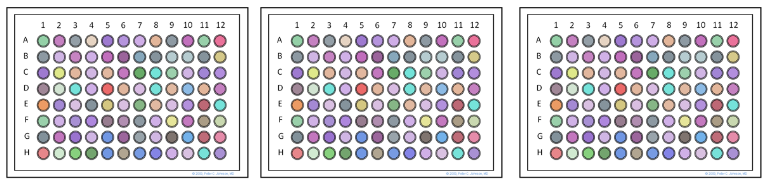
\includegraphics[width=\textwidth]{Figures/nestedplates}
\end{Exercise}

\subsection{Beyond random intercepts}

So far we have considered random effects around intercepts only (that is the meaning of the "1" in the lme4 syntax (1$\mid$ re)). But random effects can be around fixed effects. You may have heard of "random interactions", "random slopes", "random regressions"\dots


\subsection{Correlated random effects}

If we have time, ask me to talk or give examples of models with genetic or phylogenetic effects, or spatial auto-correlation.



\end{document}
